\chapter{Container as a Service with Kubernetes}
\label{cha:caas}
Container as a Service (CaaS) is a term introduced by cloud providers, which provide a cloud based container environment. But CaaS is more then just a container environment like Docker, it provides orchestration and monitoring tooling for containers, and additionally CaaS is considered to be a model for IT organizations and developers how they can build, ship and run their applications anywhere. There are multiple CaaS providers on the market, but the most popular providers are Azure Container Service, Amazon Elastic Container Service for Kubernetes (Amazon EKS) and Google Kubernetes Engine, where they bring in their own flavor of CaaS but all of them use Kubernetes beneath  \cite{CNCFKubernetes2018, MicrosoftAzureAKS2018, AmazonWebServicesEKS2018, GoogleCloudKE2018}. \\

Kubernetes is a platform for automating deployments, scaling and operation of containers across a cluster of nodes. Kubernetes provides a tooling for managing a cluster of nodes and managing the containers running on those nodes. Kubernetes has been invented by Google and is open source since 2015 and managed by the Cloud Native Computing Foundation, where the Cloud Native Computing Foundation is under the umbrella of the Linux Foundation. Kubernetes has become the most popular container orchestration tooling on the market and is used by many CaaS and PaaS providers \cite{CNCF2018}.

\section{The need for Container as a Service}
\label{sec:caas-need-for-caas}
As mentioned in \vref{sec:docker-linux-container}, running and maintaining a large set of containers becomes very hard if only the Docker is used. The deployment, scaling and management of containers must be done effortlessly, otherwise it would be almost impossible to run a large set of containers. Thus, a platform like Kubernetes is vital to enterprises and developers. Enterprises and developers need the flexibility to roll out new versions of their applications or scale them depending on the workload effortlessly. Kubernetes provides a DSL which allows to specify the infrastructure such as network, storage, CPU and RAM, as well as the build, roll out behavior and scaling of the services. Kubernetes uses the principles of IaC as discussed in Section \vref{sec:iac-principles}, therefore the service infrastructure along with the build, deployment and scaling of those service is reliable, reproducible, consistent, repeatable and disposable. The developers describe the infrastructure and behavior via the DSL, and the work is done by Kubernetes. There is the Kubernetes API Overview and lots of examples available on the Internet to get started with Kubernetes Templates \cite{CNCFKubernetesAPI2018, CNCFKubernetesGithub2018}. \\

With Kubernetes enterprises can easily implement a cluster of computing resources, build, deploy, roll out and scale their applications via a well defined workflow. This provides the possibility to fast react to new requirements of their business and an increased workload on their applications. 

\section{Kubernetes}
\label{sec:caas-kubernetes}
Kubernetes is a platform to manage containerized services in a cluster, where the Kubernetes Cluster-Nodes can be placed in the cloud or in a dedicated server infrastructure. Kubernetes is designed as a client server architecture and a master slave architecture. One node in the Kubernetes Cluster acts as the Kubernetes Master, which is discussed in Section \vref{sec:caas-kubernetes-master}, and the other nodes in the Kubernetes Cluster act as the Kubernetes Worker, which is discussed in Section \vref{sec:caas-kubernetes-worker}. The Figure \ref{fig:kubernetes-cluster-architecture} illustrates the architecture of a Kubernetes Cluster.

\begin{figure}[htbp]
	\centering
	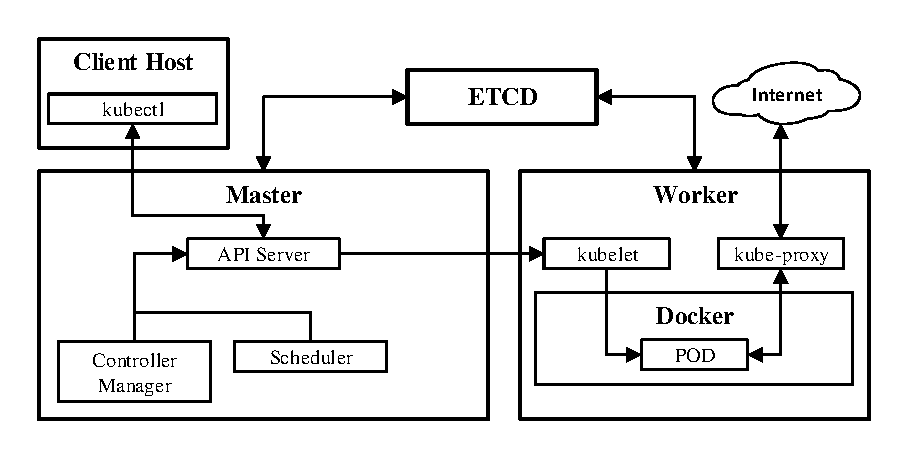
\includegraphics[scale=0.9]{images/kubernetes-cluster-architecture.pdf}
	\caption{Architecture of a Kubernetes Cluster}
	\label{fig:kubernetes-cluster-architecture}
\end{figure} 

\subsection{Kubernetes Objects}
\label{sec:caas-kubernetes-objects}
Kubernetes Objects are persistent object in the Kubernetes platform and the Kubernetes Objects describe the state of the Kubernetes cluster. The Kubernetes Cluster ensures that the state of the cluster meets the state defined by the Kubernetes Objects. The developers don't have to manually perform actions in the Kubernetes Cluster, they just have to modify the definition of the state of the Kubernetes Cluster and the Kubernetes Clusters itself will ensure that the new state definition is met by the Kubernetes Cluster. The following sections will describe some of the common used Kubernetes Objects. The overview of all Kubernetes Objects is covered by the Kubernetes API reference documentation \cite{CNCFKubernetesAPI2018}. 

\mysubsubsection{Pod}
A Pod is a group of one or more containers which are managed together. A Pod specification contains the specification for each container it bundles. All of the containers of a Pod are always scheduled on the same Kubernetes Worker and will be deployed, started and stopped as a single unit. In a pre-container world all of the applications would have been hosted on the same physical machine. A Pod allows to bundle containers together which are acting as a single service, for instance a web application container with a caching container \cite{CNCFKubernetesPods2018}. 

\mysubsubsection{Service}
A service is an abstraction which defines a set of Pods and policies how to access them. The connection to the Pod via the service abstraction is handled by the Kubernetes Proxy. The service abstraction is necessary because a Pod can be hosted on any Kubernetes Worker within the Kubernetes Cluster,  and the Pod will therefore get a random IP assigned which makes it impossible to address the Pod directly. If multiple replicas of a Pod are running, then the service will connect to a Pod of the replica set, depending on the chosen algorithm \cite{CNCFKubernetesServices2018}.

\mysubsubsection{Secret}
A secret is an abstraction to manage sensitive information which are needed by containers. A secret holds sensitive data and hides it behind a name. The secret can be referenced by a container specification by its name. A referenced secret will be injected into the container as a environment variable or a file. Therefore only the container which needs the sensitive data can access the sensitive data. 

\subsection{Kubernetes Master}
\label{sec:caas-kubernetes-master}
The Kubernetes Master is the master node in the Kubernetes Cluster. It is responsible for managing the nodes and applications running on those nodes. The Kubernetes Master exposes a REST-API via the clients can interact with the cluster. The node hosting the Kubernetes Master should be exclusively for the Kubernetes Master. The following sections briefly introduce the Kubernetes Master-Components, which are responsible for managing the Kubernetes Cluster \cite{CNCFKubernetesComponents2018}.

\mysubsubsection{Kubernetes CLI (kubectl)}
Kubectl is the CLI of Kubernetes, which provides an interface to manage the Kubernetes Cluster and an interface to manage applications running in the cluster. Kubectl is similar to the Docker CLI, but does not support direct interacting with the Docker Containers. Kubectl interacts with the Kubernetes Cluster via a REST-API exposed by the Kubernetes Master API-Server. Kubectl can be used from any client machine which can connect to the cluster without any special setup.

\mysubsubsection{Distributed Key-Value Store (etcd)}
Etcd is a distributed key-value store and provides a reliable way for sharing data within a cluster. It is the key component for the communication between the Kubernetes Master and the Kubernetes Nodes. The Kubernetes Master provides configuration for the Kubernetes Nodes and retrieves state information from the Kubernetes Nodes \cite{CoreOSETCD2018}.

\mysubsubsection{Kubernetes API-Server (kube-apiserver)}
The Kubernetes API-Server exposes the interface for interacting with the Kubernetes Cluster and is located on the Kubernetes Master Node. It represents the frontend of the Kubernetes Cluster and provides all necessary API to manage the cluster or the applications running on it.

\mysubsubsection{Kubernetes Scheduler (kube-scheduler)}
The Kubernetes Scheduler is watches the cluster for newly created Pods and assigns the Pod to node in the cluster. Multiple factors are taken into account for scheduling decisions such as individual specifications, resource requirements, available resources and hardware/policy/software constraints.

\mysubsubsection{Kubernetes Controller Manager (kube-controller-manager)}
The Kubernetes Controller Manager is responsible for the managing the different controllers. A Kubernetes Controller is running a loop and ensures that the state of the system is valid, depending on the controller type. For instance, the replication controller ensures the correct number of Pods for each replication controller object within the cluster. Kubernetes provides a set of controllers such as a replication controller, node controller, endpoint controller and service account controller.

\subsection{Kubernetes Worker}
\label{sec:caas-kubernetes-worker}
The Kubernetes Worker is a node within the Kubernetes Cluster which acts as the slave node which hosts the application containers and is managed by the Kubernetes Master. The Kubernetes Worker can be a VM or a physical machine depending on the cluster setup. It contains the Kubernetes Runtime-Environment and Docker. The following sections briefly introduce the Kubernetes Master-Components, which are responsible for managing the Kubernetes Cluster \cite{CNCFKubernetesComponents2018}. 

\mysubsubsection{Kubernetes Agent (kubelet)}
The Kubernetes Agent is a process running on the Kubernetes Worker-Nodes which interacts with the Kubernetes Master via the Kubernetes API-Server. The Kubernetes Agent ensures that the containers are running in a Pod as defined by the provided Pod specifications. The Pod specifications can be provided by an file in a specific directory (gets periodically checked), or via the Kubernetes API-Server.

\mysubsubsection{Kubernetes Network-Proxy (kube-proxy)}
The Kubernetes Network-Proxy manages the networks defined by the specifications and reflects the services which are bound to a Pod. It can perform simple TCP and UDP forwarding and can be connected to multiple backends. Any communication of a Pod to another Pod or the Internet is handled by the Kubernetes Network-Proxy. 

\mysubsubsection{Container Runtime}
The container runtime is the software responsible for running the containers on the Kubernetes Worker. Kubernetes supports multiple container runtimes, but usually its Docker which has been discussed in Chapter \vref{cha:containerization-docker}.

\section{Virtual Machine Orchestration vs Container Orchestration}
\label{sec:caas-vm-vs-container-orchestration}

